\documentclass[12pt,a4paper]{article}
\usepackage[utf8]{inputenc}
\usepackage[russian]{babel}
\usepackage[OT1]{fontenc}
\usepackage{amsmath}
\usepackage{amsfonts}
\usepackage{xcolor}
\usepackage{amsthm}
\usepackage{hyperref}
\usepackage{graphicx}
\usepackage{amssymb}
\usepackage{showkeys}
\newtheorem*{theorem*}{Теорема}
\newtheorem*{lemma*}{Лемма}
\newtheorem*{conseq*}{Следствия}
\title{Определения}
\begin{document}	
\begin{center}
Билет 1
\end{center}

Мне лень писать законы де Моргана :(

Упорядоченная пара --- это двухэлементное семейство, где множеством индексов является \{1, 2\}.

Декартовым или прямым произведением множест в X и У называется множество всех упорядоченных пар, таких что первый элемент пары принадлежит X, а второй --- Y.

\begin{center}
Билет 2
\end{center}

Аксиомы вещественных чисел:
\begin{enumerate}
\item ассоциативность сложения $(x+y)+z=x+(y+z)$
\item коммутативность сложения $x+y=y+x$
\item существование нейтрального элемента $\exists 0: x+0=0+x=x$
\item существование обратного элемента $\exists (-x): x+(-x)=(-x)+x=0$
\item ассоциативность умножения $(xy)z=x(yz)$
\item коммутативность умножения $xy=yx$
\item существование нейтрального элемента $\exists 1: x \cdot 1 = 1 \cdot x = x$
\item существование обратного элемента $\exists x^{-1}, x \ne 0: x \cdot x^{-1}= x^{-1} \cdot x = 1$
\item дистрибутивность умножения относительно сложения $x(y+z)=xy+yz$
\end{enumerate}

Так же есть аксиомы Архимеда и Кантора.

\begin{center}
Билет 3
\end{center}

Определение матматической индукции и бинома Ньютона очевидны.

Индуктивное множество --- $1 \in M$, $\forall x \in M \Rightarrow x+1 \in M$.

$\mathbb{N}$ --- минимальное по включению индуктивное подмножество $\mathbb{R}$. 

\begin{center}
Билет 4
\end{center}

Множество $E \subset \mathbb{R}$ называется \textit{ограниченным сверху/снизу}, если $\exists M \in \mathbb{R}: x \leq M$ ($x \geq M$), $x \in E$. Множество $E$ ограниченное, если оно ограничено и сверху, и снизу.

$M$ -- максимум (минимум) множества $E \subset \mathbb{R}$, если $M \in E$ и $M \geq x$ ($M \leq x$), $x \in E$. Максимум $E$ --- $\max E$, минимум $E$ --- $\min E$.

\begin{theorem*}[Существование максимума и минимума конечного множества]
\label{4.1}
Во всяком конечном подмножестве $\mathbb{R}$ есть наибольший и наименьний элемент.

Доказательство по индукции. $\blacksquare$
\end{theorem*}

\begin{conseq*}
\label{4.2}
Во всяком непустом ограниченном сверху (снизу) подмножестве $\mathbb{Z}$ есть наибольший (наименьший) элемент.
\newline
В непустом подмножестве $\mathbb{N}$ есть наименьший элемент.
\end{conseq*}

\begin{center}
Билет 5
\end{center}

Наибольшее целое число не превосходящее $x \in \mathbb{R}$ называется целой частью числа $x$ и обозначается $[x]$.

$[x] \leq x < [x] + 1$, $x - 1 < [x] \leq x$.

\begin{theorem*}[Плотность множества рациональных чисел]
\label{5.1}
Во всяком интервале есть рациональное число.

Для доказательства возьмём $a, b \in \mathbb{R}$, $a < b$. Тогда $\frac{1}{b-a} > 0$ и по аксиоме Архимеда $\exists\  n \in \mathbb{N}:\ n > \frac{1}{b-a}$, то есть $\frac{1}{n} < b-a$. Возьмём $c=\frac{[na]+1}{n}$. Тогда $c \in \mathbb{Q}$ и
\newline 
$$
c \leq \frac{na+1}{n}=a+\frac{1}{n}<a+(b-a)=b,
$$
$$
c > \frac{na-1+1}{n}=a
$$ $\blacksquare$
\end{theorem*}

\begin{conseq*}
\label{5.2}
Во всяком интервале бесконечно много рационаьных чисел.
\end{conseq*}

\begin{center}
Извилистая дорога
\end{center}

Пусть $f: X \rightarrow Y$, $A \subset X$. Образ множества $A$ при отображении $f$ --- это $$f(A)=\{y \in Y:\ \exists x \in A\ f(x)=y\}.$$

Пусть $f: X \rightarrow Y$, $B \subset Y$. Прообраз множества $B$ при отображении $f$ --- это $$f^{-1}(B)=\{x \in X: f(x) \in B\} .$$

Пусть $f: X \rightarrow Y$. Если $f(X) = Y$, то $f$ --- сюрьекция. Другими словами, для любого $Y$ есть решение в $X$.

Пусть $f: X \rightarrow Y$. Если для любых различных элементов из $X$ их образы различны, то $f$ --- инъекция.

Биекция = инъекция + сюрьекция.

Пусть $f: X \rightarrow Y$ и $f$ обратимо. Тогда обратное отображение к $f$ --- это отображение $f^{-1}$, которое каждому элементу $y$ из $f(X)$ сопоставляет (единственное) значение $x$ из $X$, для которого $f(x)=y$.

Пусть $f: X \rightarrow Y$ и $g: Y \rightarrow Z$, $f(X) \subset Y$. Тогда композиция $(g \circ f)(x)$ есть $h(x) = g(f(x))$, $x \in X$. $g$ --- внешнее отображение, $f$ --- внутреннее отображение. $f \circ g \ne g \circ f$.

\begin{center}
Билет 6
\end{center}

Два множества эквивалентны, если между ними можно провести биекцию.

Множество называется счётным, если оно эквивалентно множеству натуральных чисел.

\begin{theorem*}
\label{6.1}
Всякое бесконечное множество содержит счётное подмножество

Пусть $A$ --- бесконечное множество. В нём есть $a_1$, $A \setminus \{a_1\}$ бесконечно, поэтому в нём есть $a_2$. $A \setminus \{a_1, a_2\}$ бесконечно, поэтому в нём есть $a_3$  т.д. Новое множество $B = \{a_1, a_2, a_3, ...\}$ будет счётным по построению. $\blacksquare$
\end{theorem*}

\begin{theorem*}
\label{6.2}
Всякое бесконечное подмножество счётного подмножества счётно: $A$ счётно, $B \subset A$ и $B$ бесконечно, то $B$ --- счётно.

Расположим элементы $A$ в виде последовательности
$$
A = \{ a_1, a_2, a_3, \ldots \}
$$
Будем нумеровать элементы $B$ в порядке их появления в этой последовательности . Тем самым каждый элемент $B$ будет занумерован ровно один раз и, так как множество $B$ бесконечно, для нумерации будет использован весь натуральный ряд . $\blacksquare$
\end{theorem*}

Не более чем счётное множество --- пустое, конечное или счётное множество.

\begin{center}
Билет 7
\end{center}

\begin{lemma*}
\label{7.1}
Пусть элементы множества $A$ расположены в виде бесконечной в обоих направлениях матрице
$$
A=
\begin{pmatrix}
a_{11} & a_{12} & a_{13} & \ldots \\
a_{21} & a_{22} & a_{23} & \ldots \\
a_{31} & a_{32} & a_{33} & \ldots \\ 
\ldots & \ldots & \ldots & \ldots
\end{pmatrix}
$$
тогда $A$ счётно (для доказательства перечисляй элементы по дополнительным диагоналям).
\end{lemma*}

По лемме $\mathbb{N} \times \mathbb{N}$ --- счётно.

\begin{theorem*}
\label{7.2}
Не более чем счётное объединение не более чем счётных множеств не более чем счётно.

Пусть $B=\bigcup\limits_{k=1}^{n} A_k$ или $B=\bigcup\limits_{k=1}^{\infty} A_k$, $A_k$ не более чем счётно. Запишем элементы $A_k \setminus \bigcup\limits_{i=1}^{k-1} A_i$ в $k$-ю строку матрицы. Таким образом все клетки окажутся записаны в матрицу и по лемме выше мы получили, что $B$ эквивалентно некоторому подмножеству $\mathbb{N} \times \mathbb{N}$. $\blacksquare$
\end{theorem*}

\begin{center}
Билет 8
\end{center}

\begin{theorem*}
\label{8.1}
Множество рациональных чисел счётно.

Обозначим 
$$
\mathbb{Q}_{+} = \{x \in \mathbb{Q}: x>0\}, \mathbb{Q}_{-} = \{x \in \mathbb{Q}: x < 0\}
$$ 
При всех $q \in \mathbb{N}$ множество $\mathbb{Q}_{q} = \left\lbrace \frac{1}{q}, \frac{2}{q}, \frac{3}{q}, \ldots \right\rbrace$ счётно. По теореме 7.2 и $\mathbb{Q}_{+} = \bigcup_{q=1}^{\infty} Q_p$ счётно. Очевидно, что $\mathbb{Q}_{-} \sim \mathbb{Q}_{+}$. Снова по теореме 7.2 множество $\mathbb{Q} = \mathbb{Q}_{-} \cup \mathbb{Q}_{+} \cup {0}$ счётно. $\blacksquare$
\end{theorem*}

\begin{center}
Билет 9
\end{center}

\begin{theorem*}[Несчётность отрезка]
\label{9.1}
Отрезок $[0, 1]$ несчётен.

Допустим противное: пусть отрезок $[0, 1]$ счётен, тогда все числа в нём можно расположить в виде последовательности
$$
[0, 1] = \{ x_1, x_2, x_3, \ldots \}
$$
Разобъём отрезок $[0, 1]$ на $3$ равных отрезка $[0, \frac{1}{3}]$, $[\frac{1}{3}, \frac{2}{3}]$ и $[\frac{2}{3}, 1]$. Обозначим через $[a_1, b_1]$ тот из них, который не содержит точки $x_1$. Далее разобъём $[a_1, b_1]$ на 3 отрезка по алгоритму выше и обозначим через $[a_2, b_2]$ тот, который не содержит $x_2$. Продолжим этот процесс неограниченно. В результате получим последовательность вложенных отрезков $\{ [a_n, b_n] \}_{n=1}^{\infty}$. По аксиоме о вложенных отрезка существует точка $x^{*}$, принадлежащая всем отрезкам $[a_n, b_n]$. Также, $x^{*} \in [0, 1]$. Но тогда существует $m: x^{*}=x_m$ (по условию). По построению $x_m \not\in [a_m, b_m] \Rightarrow x^{*} \not\in [a_m, b_m]$, что противоречит принадлежности $x^{*}$ всем отрезкам. $\blacksquare$
\end{theorem*}

\begin{center}
Знак извилистой дороги
\end{center}

Пусть $\{ x_n \}_{n=1}^{\infty}$ --- последовательность вещёственных чисел. Тогда $a \in \mathbb{R}$ --- предел последовательности $\{ x_n \}$, если
$$
\forall \varepsilon>0 \ \exists N \in \mathbb{N} \ \forall n \in \mathbb{N}: n > N \  |x_n - a| < \varepsilon
$$

Пусть $V_{a}(\varepsilon) = (a-\varepsilon, a+\varepsilon)$ --- $\varepsilon$-окрестность точки $a$. Тогда $a \in \mathbb{R}$ --- предел последовательности $\{ x_n \}$, если
$$
\forall \varepsilon>0 \ \exists N \in \mathbb{N} \ \forall n \in \mathbb{N}: n > N \ x_n \in V_a(\varepsilon)
$$

Пусть $(X, \rho)$ --- метрическое пространство, $\{ x_n \}_{n=1}^{\infty}$ -- последовательность в $X$. Точку $a \in X$ называют пределом последовательности $\{ x_n \}$, если
$$
\forall \varepsilon > 0 \ \exists N \in \mathbb{N} \ \forall n \in \mathbb{N}: n > N \ \rho(x_n, a) < \varepsilon
$$

Если определения выше сильно меняются для функций и отображений, то пинганите или добавьте.

Функция $\rho: X \times X \rightarrow \mathbb{R}_{+}$ называется метрикой, если она удовлетворяет следующим условиям ($x, y, z \in X$):
\begin{enumerate}
\item $\rho(x, y) = 0 \Leftrightarrow x = y$,
\item $\rho(x, y) = \rho(y, x)$,
\item $\rho(x, y) \leq \rho(x, z) + \rho(z, y)$ (неравенство треугольника)
\end{enumerate}

Пара $(X, \rho)$ --- множество с метрикой в нём --- называется метрическим пространстом.

Пусть $K$ --- поле, $X$ --- множество, и над элементами $X$ и $K$ определены две операции: сложение $X \times X \xrightarrow{+} X$ и умножение $X \times X \xrightarrow{\cdot} X$, удовлетворяющие следующим свойстам ($x, y, z \in X$, $\gamma, \lambda \in K$):
\begin{enumerate}
\item $(x+y)+z=x+(y+z)$
\item $x+y=y+x$
\item $\exists \theta \in X: 0\cdot x = \theta$
\item $(\lambda+\gamma)x=\lambda x + \gamma x$
\item $\lambda (x+y) = \lambda x + \lambda y$
\item $(\lambda \gamma) x = \lambda (\gamma x)$
\item $1 \cdot x = x$
\end{enumerate}

Тогда $X$ --- векторное пространство над полем $K$

Пусть $X$ --- векторное пространство над $\mathbb{R}$ или $\mathbb{C}$. Нормой в $X$ называется функция $\rho: X \rightarrow \mathbb{R}_{+}$, удовлетворяющая следующим условиям:
\begin{enumerate}
\item Положительная определённость
$$
\rho(x) = 0 \Leftrightarrow x = \theta
$$

\item Положительная однородность
$$
\rho(\lambda x) = |\lambda| \rho(x)
$$

\item Неравенство треугольника (полуаддитивность)
$$
\rho(x+y) \leq \rho(x) + \rho(y)
$$
\end{enumerate}
%Я заебался это писать :((((

Норма: $\rho(x)=||x||$. Пара $(X, ||\cdot||)$ называется нормированным пространстом.

\begin{center}
Билет 10
\end{center}

\begin{theorem*}[Единственность предела последовательности]
\label{10.1}
Последовательность в в метрическом пространстве не можеть иметь более одного предела: если $x_n \rightarrow a$, $x_n \rightarrow b$, то $a=b$.

Предположим противное: пусть $a \ne b$. Тогда по первой аксиоме расстояния $\rho(a, b) > 0$. Возьмём $\varepsilon = \frac{\rho(a, b)}{2}$, по определению предела найдутся такие $N_1$ и $N_2$, что $\rho(x_n, a) < \varepsilon$ для всех $n > N_1$, а $\rho(x_n, b) < \varepsilon$ для всех $n > N_2$. Тогда, если $n>\max\{N_1, N_2\}$, то по аксиомам расстояния
$$
\rho(a, b) \leq \rho(a, x_n) + \rho(x_n, b) < \varepsilon + \varepsilon = \rho(a, b), \text{что противоречиво}
$$ $\blacksquare$
\end{theorem*}

\begin{theorem*}[Ограниченность сходящейся последовательности]
Сходящаяся последовательность ограничена

Пусть $x_n \rightarrow a$. Взяв $\varepsilon = 1$, подберём такой номер $N$, что для всех номеров $n > N$ будет $\rho(x_n, a) < 1$. Положим
$$
R = \max\{\rho(x_1, a), \ldots, \rho(x_N, a), 1\}
$$
Тогда $\rho(x_n, a) \leq R$ при всех $n \in \mathbb{N}$. $\blacksquare$
\end{theorem*}

\begin{center}
Билет 11
\end{center}

\begin{theorem*}[Предельный переход в неравенстве]
\label{11.1}
Пусть $\{ x_n \}$, $\{ y_n \}$ --- вещественные последовательности, $x_n \leq y_n$ при всех $n \in \mathbb{N}$, $a, b \in \mathbb{R}$, $x_n \rightarrow a$, $y_n \rightarrow b$. Тогда $a \leq b$. 

Предположим противное: пусть $a > b$. Тогда $\varepsilon = \frac{a-b}{2} > 0$. По определению предела найдутся такие $N_1$ и $N_2$, что $a-\varepsilon < x_n$ для всех $n > N_1$, а $y_n < b + \varepsilon$ для всех $n > N_2$. Значит, если $n > \max\{N_1, N_2\}$, то
$$
y_n < b + \varepsilon=\frac{a+b}{2}=a-\varepsilon<x_n, \text{ что противоречит условию}
$$ $\blacksquare$
\end{theorem*}

\begin{theorem*}[О сжатой последовательности]
\label{11.2}
Пусть $\{ x_n \}$, $\{ y_n \}$ и $\{ z_n \}$ --- вещественные последовательности, $x_n \leq y_n \leq z_n$ для всех $n \in \mathbb{N}$, $a \in \mathbb{R}$, $\lim x_n = \lim z_n = a$. Тогда $\lim y_n$ существует и равен $a$.

Возьмём $\varepsilon > 0$. По определению предела найдутся такие $N_1, N_2$, что $a - \varepsilon < x_n$ для всех $n > N_1$, а $z_n < a + \varepsilon$ для всех $n > N_2$. Положим $N = \max\{N_1, N_2\}$. Тогда для всех $n > N$
$$
a - \varepsilon < x_n \leq y_n \leq z_n < a + \varepsilon
$$
В силу произвольности $\varepsilon$ предел $\{y_n\}$ существует и равен $a$. $\blacksquare$
\end{theorem*}

\begin{center}
Билет 12
\end{center}

Последовательность называется бесконечно малой, если они стремится к $0$.

\begin{theorem*}(Арифметические действия над 
\newline сходящимеся последовательностями в 
\newline нормированном пространстве)
\label{12.1}
Пусть $(X, ||\cdot||)$ --- нормированное пространство, $\{ x_n \}$, $\{ y_n \}$ --- последовательности в $X$, $\{\lambda_n\}$ --- числовая последовательность, $x_0, y_0 \in X$, $x_n \rightarrow x_0$, $y_n \rightarrow y_0$, $\lambda_n \rightarrow \lambda_0$. Тогда
\begin{enumerate}
\item $x_n + y_n \rightarrow x_0 + y_0$
\item $\lambda_n y_n \rightarrow \lambda_0 y_0$
\item $x_n - y_n \rightarrow x_0 - y_0$
\item $||x_n|| \rightarrow ||x_0||$
\end{enumerate}

\begin{enumerate}
\item Возьмём $\varepsilon > 0$. По определению предела найдутся такие $N_1$ и $N_2$, что $||x_n - x_0|| < \frac{\varepsilon}{2}$ для всех $n>N_1$ и $||y_n - y_0|| < \frac{\varepsilon}{2}$ для всех $n>N_2$. Положим $N=\max\{N_1, N_2\}$. Тогда при всех $n > N$ будет
$$
|| (x_n + y_n) - (x_0 + y_0) || < || x_n - x_0 || + || y_n - y_0 || < \frac{\varepsilon}{2} + \frac{\varepsilon}{2} = \varepsilon
$$

\item По неравенству треугольника 
$$
|| \lambda_n x_n - \lambda_0 x_0 || = || (\lambda_n - \lambda_0) x_n + \lambda_0 (x_n - x_0) || \leq
$$
$$
\leq |\lambda_n - \lambda_0| || x_n || + |\lambda_0|	||x_n - x_0||
$$
По условию последовательности $\{|\lambda_n - \lambda_0|\}$, $\{|x_n - x_0|\}$ бесконечно малые, а по теореме 10.2 последовательность $\{||x_n||\}$ ограничена, как и постоянная последовательность $\{|\lambda_0|\}$. Следовательно по лемме "Произведение бесконечно малой последовательности на ограниченную есть бесконечно малая" оба слагаемых в правой части бесконечно малые, а тогда по утверждению 1 их сумма бесконечно малая. Наконец, $||\lambda_n x_n - \lambda_0 x_0||\rightarrow 0$ по теореме 11.1.

\item Доказывается аналогично утверждению 1 или применением уже доказанных утверждений 1 и 2:
$$
x_n - y_n = x_n + (-1) y_n \rightarrow x_0 + (-1) y_0 = x_0 - y_0
$$

\item Утверждение следует из неравенства
$$
\big\vert \Vert x_n \Vert - \Vert x_0 \Vert \big\vert \leq \Vert x_n - x_0 \Vert
$$
(леммы про свойства полунорм) и теоремы 11.1.
\end{enumerate}
$\blacksquare$
\end{theorem*}

\begin{center}
Билет 13
\end{center}

Пусть $X$ --- векторное пространство над $\mathbb{R}$ или $\mathbb{C}$. Функция $\phi: X \times X \rightarrow \mathbb{R} (\mathbb{C})$ называется скалярным произведением в $X$ (обозначение: $\phi(x, y) = (x, y)$), если она удовлетворяет следующим аксиомам:
\begin{enumerate}
\item Линейность по первому аргументу
$$
(\lambda x_1 + \mu x_2, y) = \lambda (x_1, y) + \mu (x_2, y)
$$

\item Эрмитовская симметричность
$$
(y, x) = \overline{(x, y)}
$$

\item Положительная определённость
$$
(x, y) \geq 0; (x, x) = 0 \Leftrightarrow x=\theta
$$
\end{enumerate}

Свойства скалярного произведения:
\begin{enumerate}
\item $(x, y_1 + y_2) = (x, y_1) + (x, y_2)$
\item $(x, \lambda y) = \overline{\lambda} (x, y)$
\item $(\theta, y) = (x, \theta) = 0$
\end{enumerate}

\begin{theorem*}{Неравенство Коши-Буняковского-Шварца}
\label{13.1}
$$
{|(x, y)|}^2 \leq (x, x) (y, y)
$$

Пусть $(y, y) > 0$ (в противном случае $y=\theta$ и неравенство выполнено), положим
$$
\lambda = -\frac{(x, y)}{(y, y)}
$$
Тогда в силу аксиом скалярного произведения и равенства $\lambda \overline{\lambda} = {|\lambda|}^2$
\begin{align*}
(x + \lambda y, x + \lambda y) &= (x, x) + \overline{\lambda} (x, y) + \lambda (y, x) + {|\lambda|}^2 (y, y) = \\
&=(x,x) -  \frac{{|(x, y)|}^2}{(y, y)}-\frac{{|(x, y)|}^2}{(y, y)}+\frac{{|(x, y)|}^2}{(y, y)}
\end{align*}
Таким образом,
$$
(x, x) (y, y) - {|(x, y)|}^2 = (y, y) (x + \lambda y, x+\lambda y) \geq 0
$$
$\blacksquare$
\end{theorem*}

\begin{lemma*}[Это не лемма, просто хз как обозвать]
\label{13.2}
Функция $\rho(x) = \sqrt{(x, x)}$ --- норма в $X$.

Положительная определённость $\rho$ следует из положительной определённости скалярного произведения. Далее,
$$
\rho(\lambda x) = \sqrt{(\lambda x, \lambda x)} = \sqrt{\lambda \overline{\lambda} (x, x)} = |\lambda| \rho(x)
$$
Докажем неравенство треугольника. Применяя 13.1, имеем
\begin{align*}
{\rho}^2 (x+y) &=(x+y, x+y) = (x, x) + (x, y) + (y, x) + (y, y) = \\
&=(x, x) + 2Re(x, y) + (y, y) \leq (x,x) + 2|(x, y)| + (y, y) \leq  \\
&\leq {\rho}^2 (x) + 2\rho(x)\rho(y) + {\rho}^2(y) = {(\rho(x)+\rho(y))}^2 \ \blacksquare
\end{align*}
\end{lemma*}

\begin{center}
Билет 14
\end{center}

\begin{conseq*}(КБШ в $\mathbb{R}^m$ и $\mathbb{C}^m$)
\label{14.1}
\begin{enumerate}
\item Скалярное произведение в $\mathbb{R}^m$:
$$
(x, y) = \sum\limits_{k=1}^{m} x_k y_k
$$

\item Скалярное произведение в $\mathbb{C}^m$:
$$
(z, w) = \sum\limits_{k=1}^{m} z_k \overline{w_k}
$$

$\blacksquare$
\end{enumerate}
\end{conseq*}

Далее запись $x_{i}^{(j)}$ подразумевает, что $i$ --- номер координаты, $j$ --- номер последовательности.

Говорят, что последовательность $\{ x^{(n)} \}$ точек $\mathbb{R}^m$  сходится к пределу $x^{(0)} \in \mathbb{R}^m$ покоординатно, если $x_{j}^{(n)} \xrightarrow[n\rightarrow \infty]{} x_{j}^{(0)}$, для всех $j \in [1:m]$.

\begin{lemma*}
\label{14.2}
В $\mathbb{R}^m$ покоординатная сходимость и сходимость по Евклидовой норме равносильны.

Утверждение следует из неравенств
\begin{align*}
|x_{j}^{(n)} - x_{j}^{(0)}| \leq & |x^{(n)} - x^{(0)}| = \\
= & \sqrt{\sum\limits_{k=1}^{m} {(x_{k}^{(n)} - x_{k}^{(0)})}^2} \leq \sqrt{m} \max\limits_{1\leq k \leq m} {|x_{k}^{(n)}-x_{k}^{(0)}|}
\end{align*}
и теоремы 11.1. $\blacksquare$
\end{lemma*}

\begin{center}
Билет 15
\end{center}

Говорят, что вещественная последовательность $\{x_n\}$ стремится к:
\begin{enumerate}
\item плюс бесконечности, если 
$$
\forall E>0\ \exists N \in \mathbb{N}\ \forall n \in \mathbb{N}: n > N\ x_n > E
$$
\item минус бесконечности ($x_n < -E$)
\item бесконечности (бесконечности неопределённого знака) ($|x_n| > E$)
\end{enumerate}

Последовательность, стремящаяся к бесконечности называется бесконечно большой.

\begin{theorem*}[Арифметические действия над бесконечно большими]
\label{15.1}
Пусть $\{x_n\}$, $\{y_n\}$ --- числовые последовательности
\begin{enumerate}
\item Если $x_n\rightarrow +\infty$, $\{y_n\}$ ограничена снизу, то $x_n+y_n\rightarrow +\infty$

\item Если $x_n\rightarrow -\infty$, $\{y_n\}$ ограничена сверху, то $x_n+y_n\rightarrow -\infty$

\item Если $x_n\rightarrow \infty$, $\{y_n\}$ ограничена, то $x_n+y_n\rightarrow \infty$

\item Если $x_n\rightarrow \pm\infty$, $y_n \geq b > 0$ для всех $n$ (или $y_n \rightarrow b_1 > 0$), то $x_n y_n \rightarrow \pm\infty$

\item Если $x_n\rightarrow \pm\infty$, $y_n \leq b < 0$ для всех $n$ (или $y_n \rightarrow b_1 < 0$), то $x_n y_n \rightarrow \mp\infty$

\item Если $x_n\rightarrow \infty$, $|y_n| \geq b > 0$ для всех $n$ (или $y_n \rightarrow b_1 \ne 0$), то $x_n y_n \rightarrow \infty$

\item Если $x_n \rightarrow a \ne 0$, $y_n \rightarrow 0$, $y_n \ne 0$ при всех $n$, то $\frac{x_n}{y_n} \rightarrow \infty$

\item Если $x_n \rightarrow a \in \mathbb{C}$, $y_n \rightarrow \infty$, то $\frac{x_n}{y_n} \rightarrow 0$

\item Если $x_n \rightarrow \infty$, $y_n \rightarrow b \in \mathbb{C}$, $y_n \ne 0$ при всех $n$, то $\frac{x_n}{y_n} \rightarrow \infty$
\end{enumerate}

Почти всё очевидно, докажем 8 пункт для наглядности.

По теореме о пределе произведения и лемме ``Последовательность бесконечно большая, когда обратная ей бесконечно малая`` получаем, что
$$
\frac{x_n}{y_n} = x_n \cdot \frac{1}{y_n} \rightarrow a \cdot 0 = 0 \blacksquare
$$
\end{theorem*}

\begin{center}
Знак извилистой дороги
\end{center}

Точка $a$ называется внутренней точкой множества $D$, если существует окрестность точки $a$, содержащаяся в $D$.

Множество $D$ называется открытым, если все его точки внутренние.

Множество $D$ называется замкнутым в $X$, если оно содержит все свои предельные точки.

Подмножество $K$ метрического пространства $X$ называется компактным, если из любого открытого покрытия $К$ можно извлечь конечное подпокрытие:
$$
\forall \{G_a\}_{a\in A}: K \subset \bigcup\limits_{a\in A} G_a, G_a \text{ открыты в } X
$$

\begin{center}
Билет 16
\end{center}

\begin{theorem*}[Свойства открытых множеств]
\label{16.1}
\ %это надо для красивого отступа 
\begin{enumerate}
\item Объединение любого семейства открытых множеств открыто. 

Пусть задано семейство открытых множеств $\{G_a\}_{a \in A}$, $G = \bigcup\limits_{a\in A}{G_a}$, $x \in G$. Докажем, что $x$ --- внутренняя точка $G$. В самом деле, по определению объединения найдётся такой индекс $a$, что $x \in G_a$. Так как $G_a$ открыто, $x$ --- внутренняя точка этого шара, значит существует шар $B(x, r)$, содержащийся в $G_a$. Но тогда тем более $B(x, r) \subset G$.

\item Пересечение конечного семейства открытых множеств открыто. 

Пусть задано конечное семейство открытых множеств $\{G_k\}_{k=1}^{n}$, $G = \bigcap\limits_{k=1}^{n} G_k$, $x \in G$. Тогда $x$ принадлежит каждому из множеств, и в силу открытости $G_k$ найдутся такие положительные числа $r_1, \ldots, r_n$, что $B(x, r_k) \in G_k$ при всех $k \in [1: n]$. Обозначим $r=\min\{r_1, \ldots, r_n\}$, тогда $B(x, r) \in G_k$ для всех $k$. Следовательно по определению пересечения $B(x, r) \in G$. $\blacksquare$
\end{enumerate}
\end{theorem*}

\begin{lemma*}[Открытый шар открыт]
\label{16.2}
Покажем, что шар $B(a, r)$ открыт. Пусть $p \in B(a, r)$, то есть $\rho(p, a) < r$.
\begin{center}
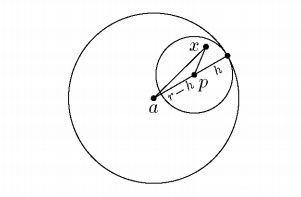
\includegraphics[scale=0.7]{openCircle.jpg}
\end{center}
Докажем, что $p$ --- внутренняя точка шара. Положим $h = r - \rho(p, a)$ ($h > 0$) и проверим, что $B(p, h) \subset B(a, r)$. Пусть $x \in B(p, h)$, то есть $\rho(x, p) < h$. Тогда
$$
\rho(x, a) \leq \rho(x, p) + \rho(p, a) < h + r - h = r
$$
То есть $x \in B(a, r)$. $\blacksquare$
\end{lemma*}

Множество всех внутренних точек множества $D$ называется внутренностью $D$ и обозначается $\stackrel{\circ}{D}$ или $Int\ D$.

\begin{center}
Билет 17
\end{center}

Точка $a$ называется предельной точкой множества $D$, если в любой окрестности точки $a$ найдётся точка $D$, отличная от $a$. Другими словами, если $\stackrel{.}{V_a} \cap D \ne \emptyset$.

\begin{theorem*}[Связь открытости и замкнутости]
\label{17.1}
Множество открыто тогда и только тогда, когда его дополнение замкнуто

Пусть $D^c$ замкнуто. Возьмём точку $x \in D$ и докажем, что $х$ --- внутренняя точка $D$; в силу произвольности $x$ это и будет означать, что $D$ открыто. Поскольку $x \not\in D^c$, а $D^c$ замкнуто, $x$ не является предельной точкой $D^c$, то есть существует такая окрестность $V_x$ точки $х$, что $\stackrel{\cdot}{V_x} \cap D = \emptyset$. Тогда и $V_x \cap D^c = \emptyset$, так как $x \in D$. Но это означает, что $V_x \subset D$, то есть $x$ --- внутренняя точка $D$.

Пусть $D$ открыто. Возьмём точку $x$, предельную для $D^c$, и докажем, что $x \in D^c$; в силу произвольности $x$ это и будет означать, что $D^c$ замкнуто. Поскольку в любой окрестности точки $x$ найдётся точка $D^c$, $x$ не является внутренней точкой $D$, а тогда, в силу открытости $D$, $x \not\in D$, то есть $x \in D^C$. $\blacksquare$
\end{theorem*}

\begin{theorem*}[Свойства замкнутых множеств]
\label{17.2}
\ 
\begin{enumerate}
\item Пересечение любого семейства замкнутых множеств замкнуто.
\item Объединение конечного семейства замкнутых множеств замкнуто.
\end{enumerate}

Доказательство следует из 17.1 и этих формул.
$$
\bigcap\limits_{a\in A}{F_a} = {\left( \bigcup\limits_{a\in A}{F_{a}^{c} }\right)}^{c}, \bigcup\limits_{k=1}^{n}{F_a} = {\left( \bigcap\limits_{k=1}^{n}{F_{a}^{c} }\right)}^{c} \blacksquare
$$
\end{theorem*}

Замыкание $D$ есть множество всех точек прикосновения. Обозначается $\overline{D}$ или $Cl\ D$.

\begin{center}
Билет 18
\end{center}

\begin{theorem*}[Открытость и замкнутость в пространстве]
\label{18.1}
Пусть $(X, \rho)$ --- метрическое пространство, $D \subset Y \subset X$.
\begin{enumerate}
\item $D$ открыто в $Y$ тогда и только тогда, когда существует такое множество $G$, открытое в $X$, что $D = G \cap Y$

Пусть $D=Y\cap G$, где $G$ открыто в $X$. Возьмём точку $a \in D$. В силу открытости $G$ в $X$ существует окрестность $V_{a}^{X}$ точки $a$ в $X$: $V_{a}^{X} \subset G$. Тогда $V_{a}^{Y}=V_{a}^{X} \cap Y$ --- окрестность $a$ в $Y$ и $V_a^{Y} \subset D$. Значит, $a$ --- внутренняя точка $D$. В силу произвольности $a$ множество $D$ открыто в $Y$.

Обратно, пусть $D$ открыто в $Y$. Тогда для каждой точки $a \in D$ найдётся её окрестность в $Y$, содержащаяся в $D$: $V_{a}^{Y} = B^{Y}(a, r_a) \subset D$. Обозначим $G = \bigcup\limits_{a\in D}{B^{X}(a, r_a)}$. Тогда $G$ открыто в $X$ как обхединения открытых в $X$ множеств, и
$$
G\cap Y = \bigcup\limits_{a\in D}{(B^{X}(a, r_a) \cap Y} = \bigcup\limits_{a \in D}{B^{Y}(a, r_a)} = D
$$

\item $D$ замкнуто в $Y$ тогда и только тогда, когда существует такое множество $F$, замкнутое в $X$, что $D = F \cap Y$

По теореме 17.1 замкнутость $D$ в $Y$ равносильна открытости $Y \setminus D$ в $Y$. По доказанному последнее равносильно существованию такого открытого в $X$ множества $G$, что $Y \setminus D = G \cap Y$. Осталось обозначить $F = G^{c}$ и учесть, что соотношения $D = F \cap Y$ и $Y \setminus D = G \cap Y$ равносильны. $\blacksquare$
\end{enumerate}
\end{theorem*}

\begin{center}
Билет 19
\end{center}

\begin{lemma*}
\label{19.1}
Пусть $(X, \rho)$ ---  метрическое пространство, $Y$ --- подпространство $X$, $K \subset Y$. Тогда свойства компактности $K$ в $X$ и $Y$ равносильны

Пусть $K$ компактно в $X$. Возьмём покрытие $K$ множествами $V_a$, открытыми в $Y$. По теореме 18.1 $V_a = G_a \cap Y$, где множества $G_a$ открыты в $X$. Множества $G_a$ образуют покрытие $K$:
$$
K \subset \bigcup\limits_{a\in A}{V_a} \subset \bigcup\limits_{a \in A}{G_a}
$$
Пользуясь компактностью $K$ в $X$, извлечём покрытия $\{G_{a}\}_{a\in A}$ конечное подпокрытие: $K\subset \bigcup\limits_{i=1}^{N}{G_{a_i}}$. Но, поскольку $K \subset Y$,
$$
K \subset \bigcup\limits_{i=1}^{N}{(G_{a_i} \cap Y)} = \bigcup\limits_{i=1}^{N} V_{a_i}
$$
Итак, из произвольного покрытия $K$ множествами, открытыми в $Y$, можно извлечь конечное подпокрытие, что и означает компактность $K$ в $Y$.

Пусть теперь $K$ помпактно в $Y$. Возьмём покрытие $K$ множествами $G_a$, открытыми в $X$. Положим $V_a = G_a \cap Y$; тогда множества $V_a$ открыты в $Y$ и образуют покрытие $K$. В силу компактности $K$ в $Y$ из него можно извлечь конечное подпокрытие $\{V_{a_i}\}_{i=1}^{N}$. Но тогда $\{G_{a_i}\}_{i=1}^{N}$ --- тоже покрытие $K$, и компактность $K$ в $X$ доказана. $\blacksquare$
\end{lemma*}

\begin{center}
Билет 20
\end{center}

\begin{theorem*}[Простейшие свойства компактов]
\label{20.1}
Пусть $(X, \rho)$ --- метрическое пространство, $K \subset X$.
\begin{enumerate}
\item Если $K$ компактно, то $K$ замкнуто и ограничено

Докажем, что $K^c$ открыто. Возьмём точку $a \in K^c$ и покажем, что $a$ --- внутренняя точка $K^c$; в силу произвольности $a$ это и  будет означать, что $K^c$ открыто. Для каждой точки $q \in K$ положим
$$
r_q = \frac{\rho(q, a)}{2}, V_q = B(a, r_q), W_q = B(q, r_q)
$$
Тогда $V_q \cap W_q = \emptyset$. Семейство $\{W_q\}_{q\in K}$ --- открытое покрытие компакта $K$. Извелечём из него конечное подпокрытие $\{W_{q_i}\}_{i=1}^{N}$: $K\subset \bigcup\limits_{i=1}^{N}{W_{q_i}} = W$. Тогда $V = \bigcap\limits_{i=1}^{N}{V_{q_i}}$ --- окрестность точки $a$, причём $V \cap W = \emptyset$. Тем более $V \cap K = \emptyset$, то есть $V \subset K^c$.

Докажем, что $K$ ограничено. Зафиксируем точку $a \in X$ и рассмотрим покрытие множества $K$ открытыми шараиш $\{B(a, n)\}_{n=1}^{\infty}$. В силу компактности $K$ покрывается конечным набором шаров $\{B(a, n_i)\}_{i=1}^{N}$ и, следовательно, содержится в шаре $B\left(a, \max\limits_{1\leq i \leq N}{n_i} \right)$

\item Если $X$ компактно, а $K$ замкнуто, то $K$ компактно

Пусть $\{G_a\}_{a\in A}$ --- открытое покрытие $K$. Тогда, поскольку $K$ замкнуто, $\{G_a\}_{a\in A} \cup\{K^c\}$ --- открытое покрытие $X$. Пользуясь компактностью $X$, извлечём из него конечное подпокрытие $X$: $X=\bigcup\limits_{i=1}^{N}{G_{a_i} \cup K^C}$. Но тогда $\{G_{a_i}\}_{i=1}^{N}$ --- покрытие $K$. $\blacksquare$
\end{enumerate}
\end{theorem*}

\end{document}